\clearpage
\begin{flushright}
  \fechaclase{21 de septiembre de 2026}
\end{flushright}

\subsection{SMC con atenuación de Chattering}

Sea el sistema no lineal
\[
  \dot{x}=f(x,t)+u
\]
\[
  y=x
\]
Se propone la siguiente superficie de deslizamiento para el seguimiento de
trayectorias
\[
  \sigma=e+m\int e\,dt
\]
donde $m>0$ es una constante de diseño. Verificamos la dinámica dse la
superficie
\[
  e+m\int e\,dt=0
\]
\[
  e(t)=e(0)\exp(-mt)
\]
lo que garantiza convergencia asintótica. Derivando la superficie
\[
  \dot{\sigma}=\dot{e}+me
\]
\[
  \dot{\sigma}=me+\dot{r}-f(x,t)-u
\]

Se propone la función de Lyapunov
\[
  V=\frac{1}{2}\sigma^2
\]
y su derivada
\[
  \dot{V}=\sigma\dot{\sigma}
  =\sigma\left[me-\dot{r}-f(x,t)-u\right]
\]
\[
  \dot{V}=m\sigma e-\sigma\left[\dot{r}+f(x,t)\right]-\sigma u
\]
\[
  \dot{V}\leq m\lvert e\rvert\lvert\sigma\rvert
  +L\lvert\sigma\rvert-\sigma u
\]

Asumiendo la cota
\[
  \left\lvert\dot{r}+f(x,t)\right\rvert\leq L,
\]
se propone el controlador
\[
  u=K V_{eq}\operatorname{sign}(\sigma)
\]

\[
  \dot{V}\leq(m\lvert e\rvert+L)\lvert\sigma\rvert
  -K V_{eq}\lvert\sigma\rvert
\]
Si
\[
  V_{eq}=-m\lvert e\rvert+L
\]
\[
  \dot{V}\leq
  \left[m\lvert e\rvert+L-K(m\lvert e\rvert+L)\right]
  \lvert\sigma\rvert
\]
\[
  \dot{V}\leq-(K-1)\lvert\sigma\rvert
\]
Haciendo $K>1$, el sistema es estable.

\paragraph{\tituloejemplo{Ejemplo}}
Aplique el controlador al sistema
\[
  \dot{x}=2\operatorname{sen}(x)\cos(x)+u
\]
\[
  y=x
\]
\[
  V_{eq}=m\lvert e\rvert+2
\]
\[
  \sigma=e+m\int e\,dt
\]
\[
  u=K V_{eq}\operatorname{sign}(\sigma)
\]

\paragraph{Resolución}

El controlador se implementa dentro de un bloque \texttt{MATLAB Function}:

\begin{MatlabCode}
function u = controlador(e, ie)

% Ganancia K>1
K = 3;

% Valor arbitrario positivo
m = 4;

Veq = m*abs(e)+2;
sigma = e + m*ie;
u = K*Veq*sign(sigma);

\end{MatlabCode}

La planta también se implementa dentro de un bloque
\texttt{MATLAB Function}:

\begin{MatlabCode}
function [dx,y] = planta(x, u)

dx = 2*sin(x)*cos(x) + u;
y = x;
\end{MatlabCode}

\begin{center}
  \href{file:../../sim/Parcial\%201/}{%
    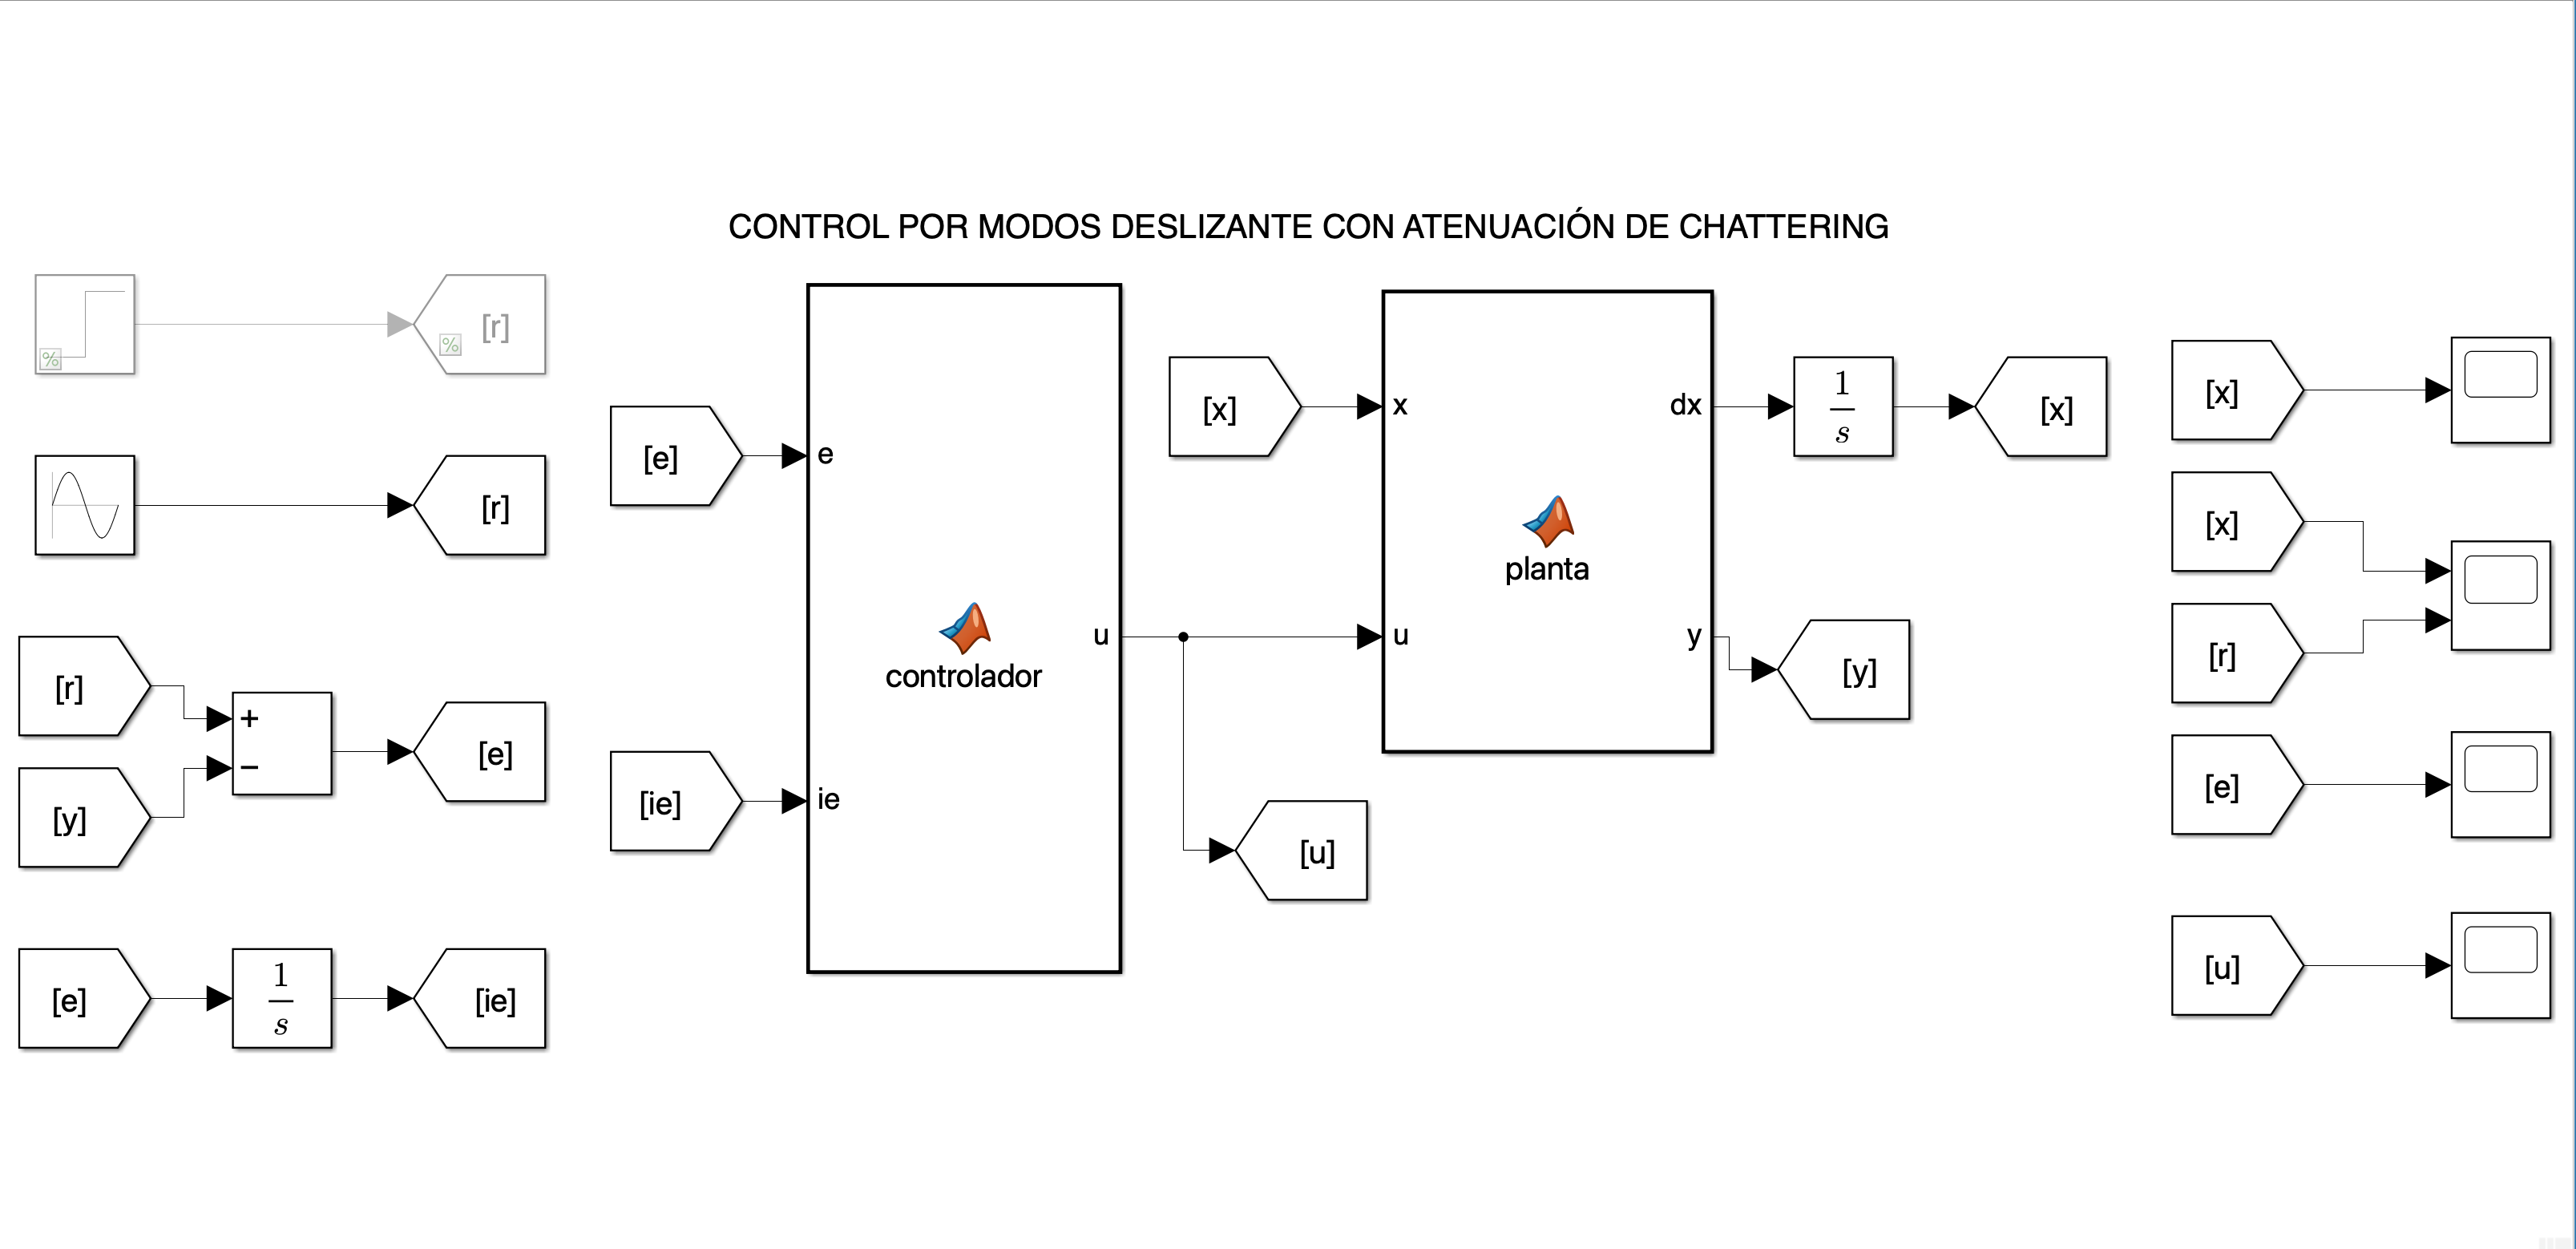
\includegraphics[width=0.85\textwidth]{img/SMC_atenuacionChattering_seg_tray_V1.png}%
  }

  \small\textit{Haga clic en la imagen para abrir la carpeta de los modelos de Simulink y abra el archivo \texttt{EjemploSMC\_seg\_tray\_atenuacion\_chattering\_V1.slx} para ejecutar la simulación.}
\end{center}
